
\documentclass[journal] {article}


%\usepackage{graphics}
\usepackage{graphicx}


\begin{document}

\title{demo document}
\maketitle

\section{first}

ugjcjgvjv igkgig
kgkvkjbvkjbjbjbb kjbkjbkjbjb jjjjjjjjjjjjjjjjjjjjjjjjjjjjjjjjjjjjjjjjjjjj jjjjjjjjjjjjjjjjjjj jjjjjjjjjjjjjjjjj
gggggggggggggggggg hhhhhhhhhhhhhhhhhhhhhhhh hhhhhhhhhhhhhhhhhhhhhhhh

jjjjjjjjjjjjjjjjjjjjjjjjjjjjjjjjjjjjjjjjjj jjjjjjjjjjjjjjjjjjjjjjjjjjjjjjjj jjjjjjjjjjjjjjjjjjjjjjjjj


\begin{itemize}
	\item aaaaaaaaaaaaaaaaaaaaaaaaa
	\item bbbbbbbbbbbbbbbbbbbbbbbbb
\end{itemize}



\begin{enumerate}
	\item aaaaaaaaaaaaaaaaaaaaaaaaaaaaa
	\item bbbbbbbbbbbbbbbbbbbbbbbb
\end{enumerate}




\begin{description}
	\item[step 1] aaaaaaaaaaaaaaaaaaaaaaaaaaaaaaa
	\item [step 2] bbbbbbbbbbbbbbbbbbbbbbbbbbbbbbb
\end{description}




\begin{figure}[htbp]
	\centering
		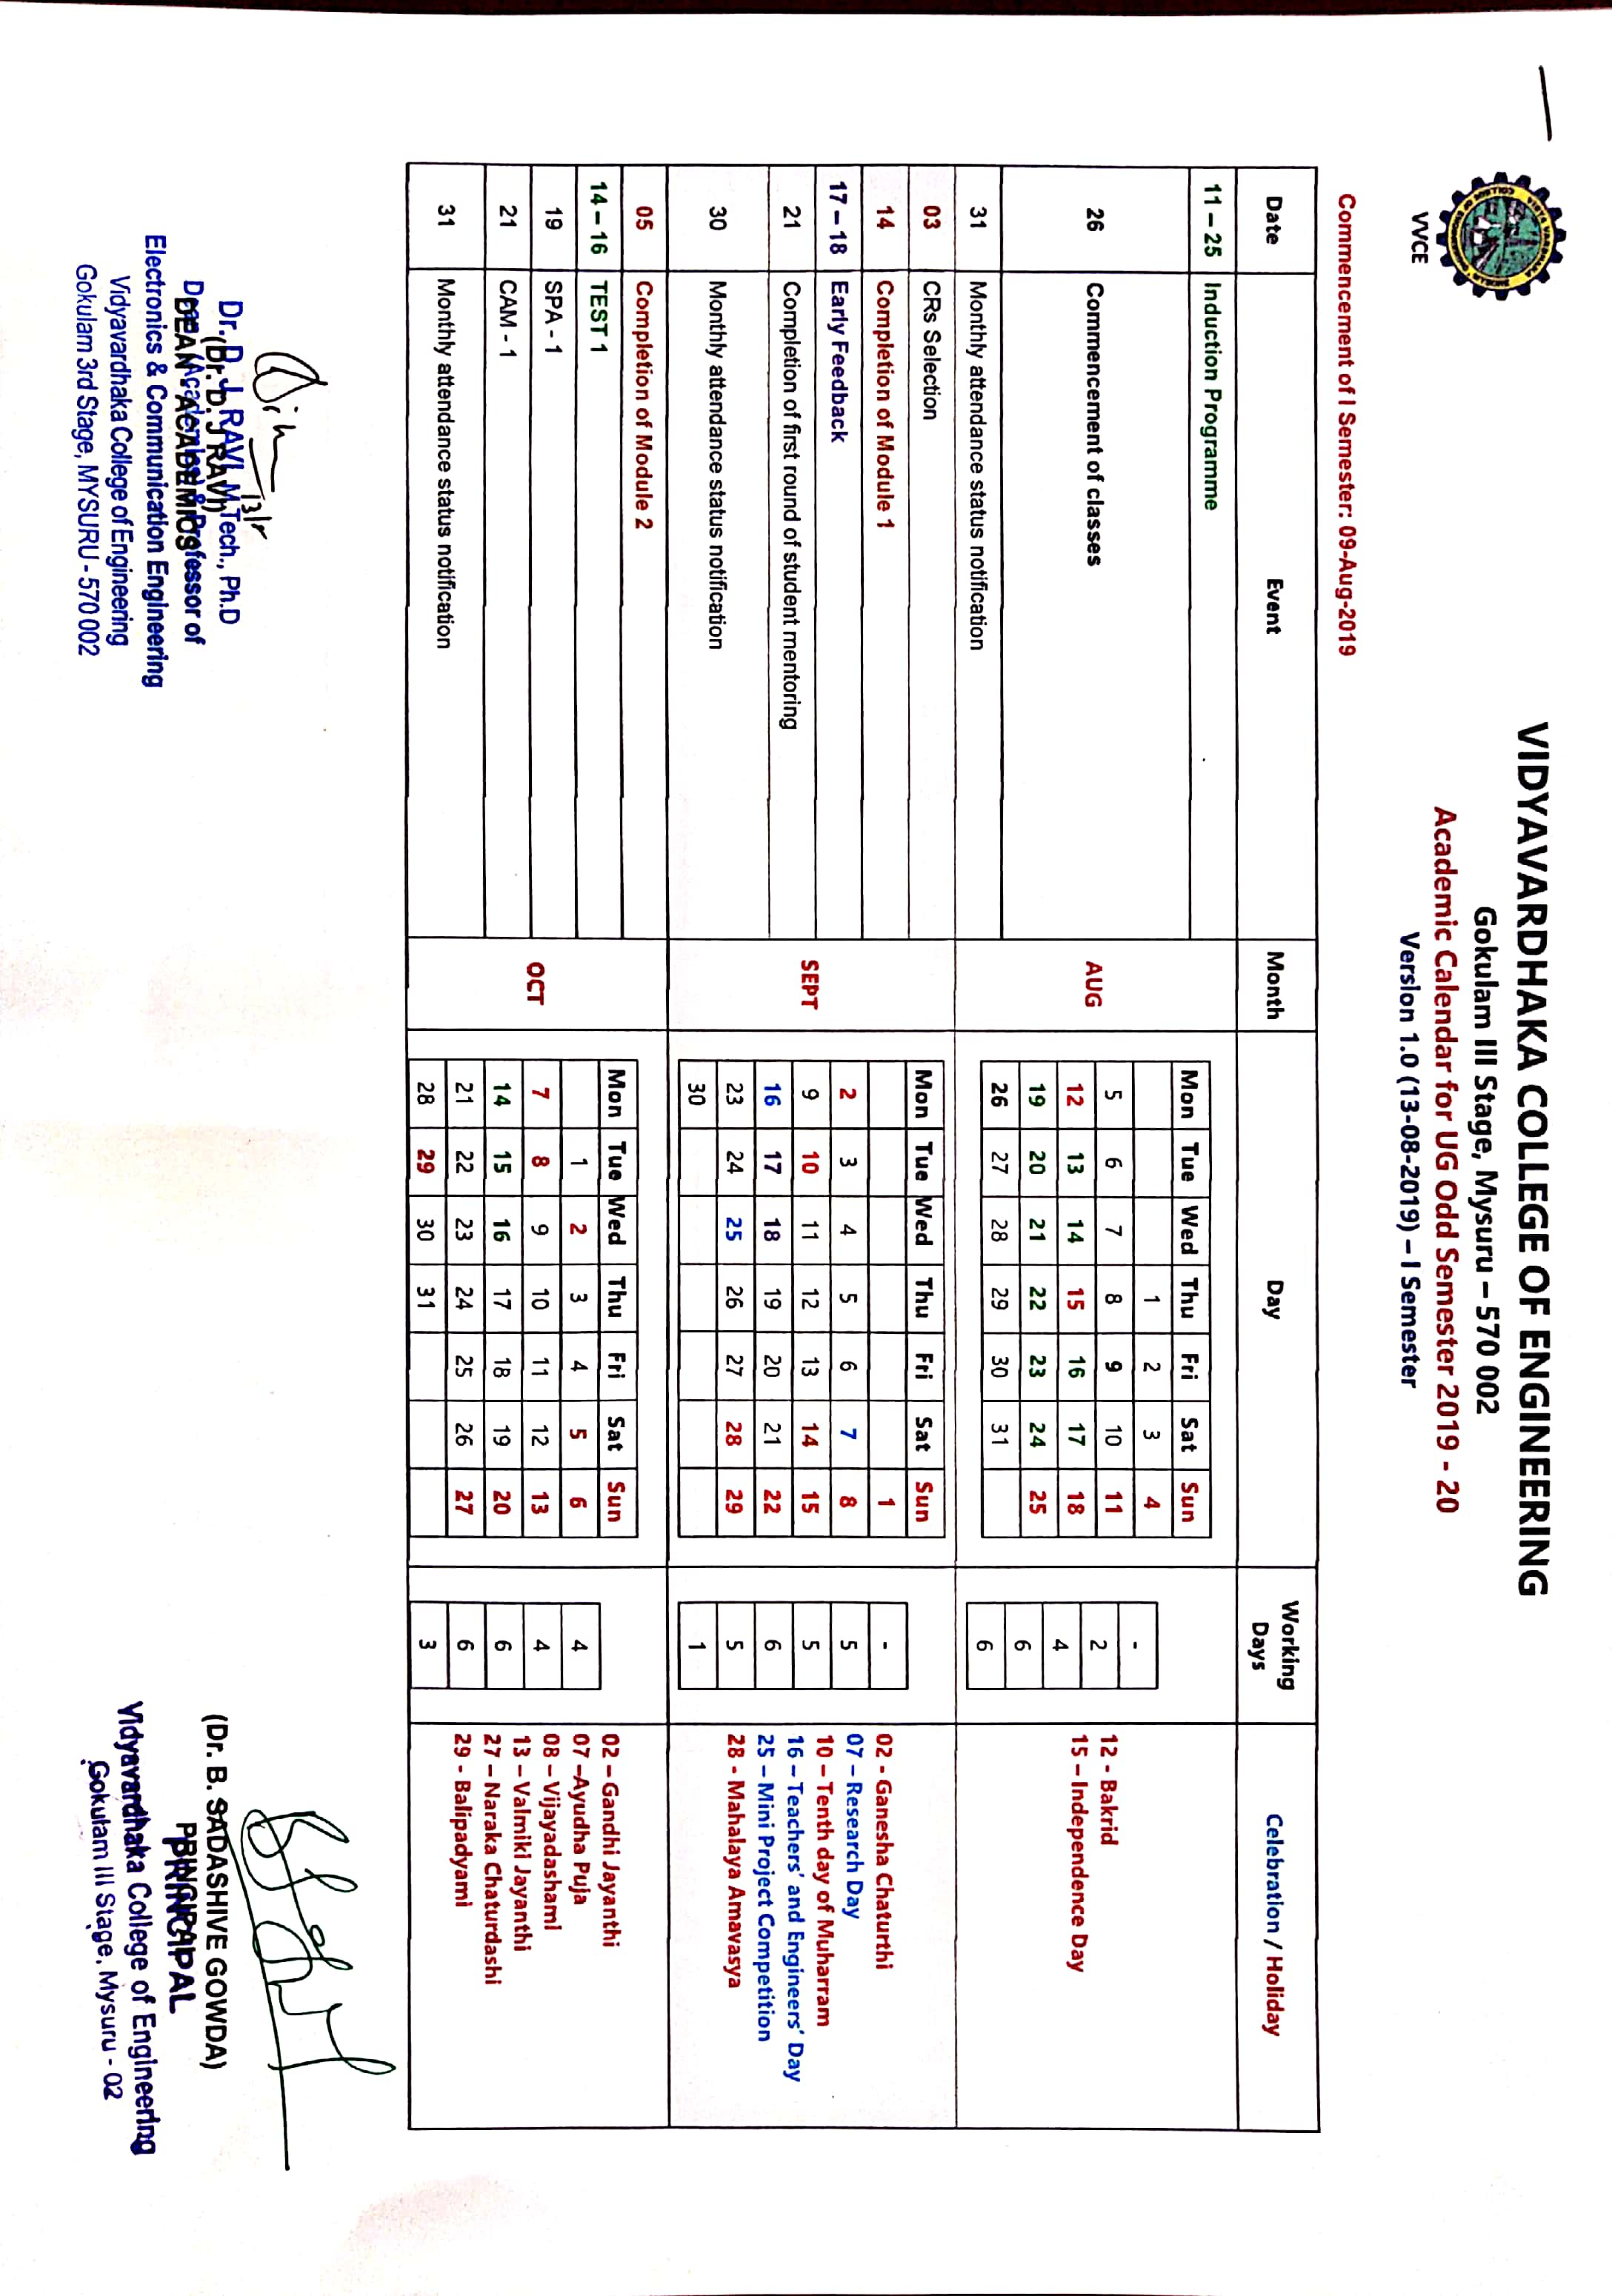
\includegraphics{CoE-1st Sem-Page1.jpg}
	\caption{sample figure}
	\label{fig:CoE-1st Sem-Page1}
\end{figure}


\begin{figure}[t]
	\centering
		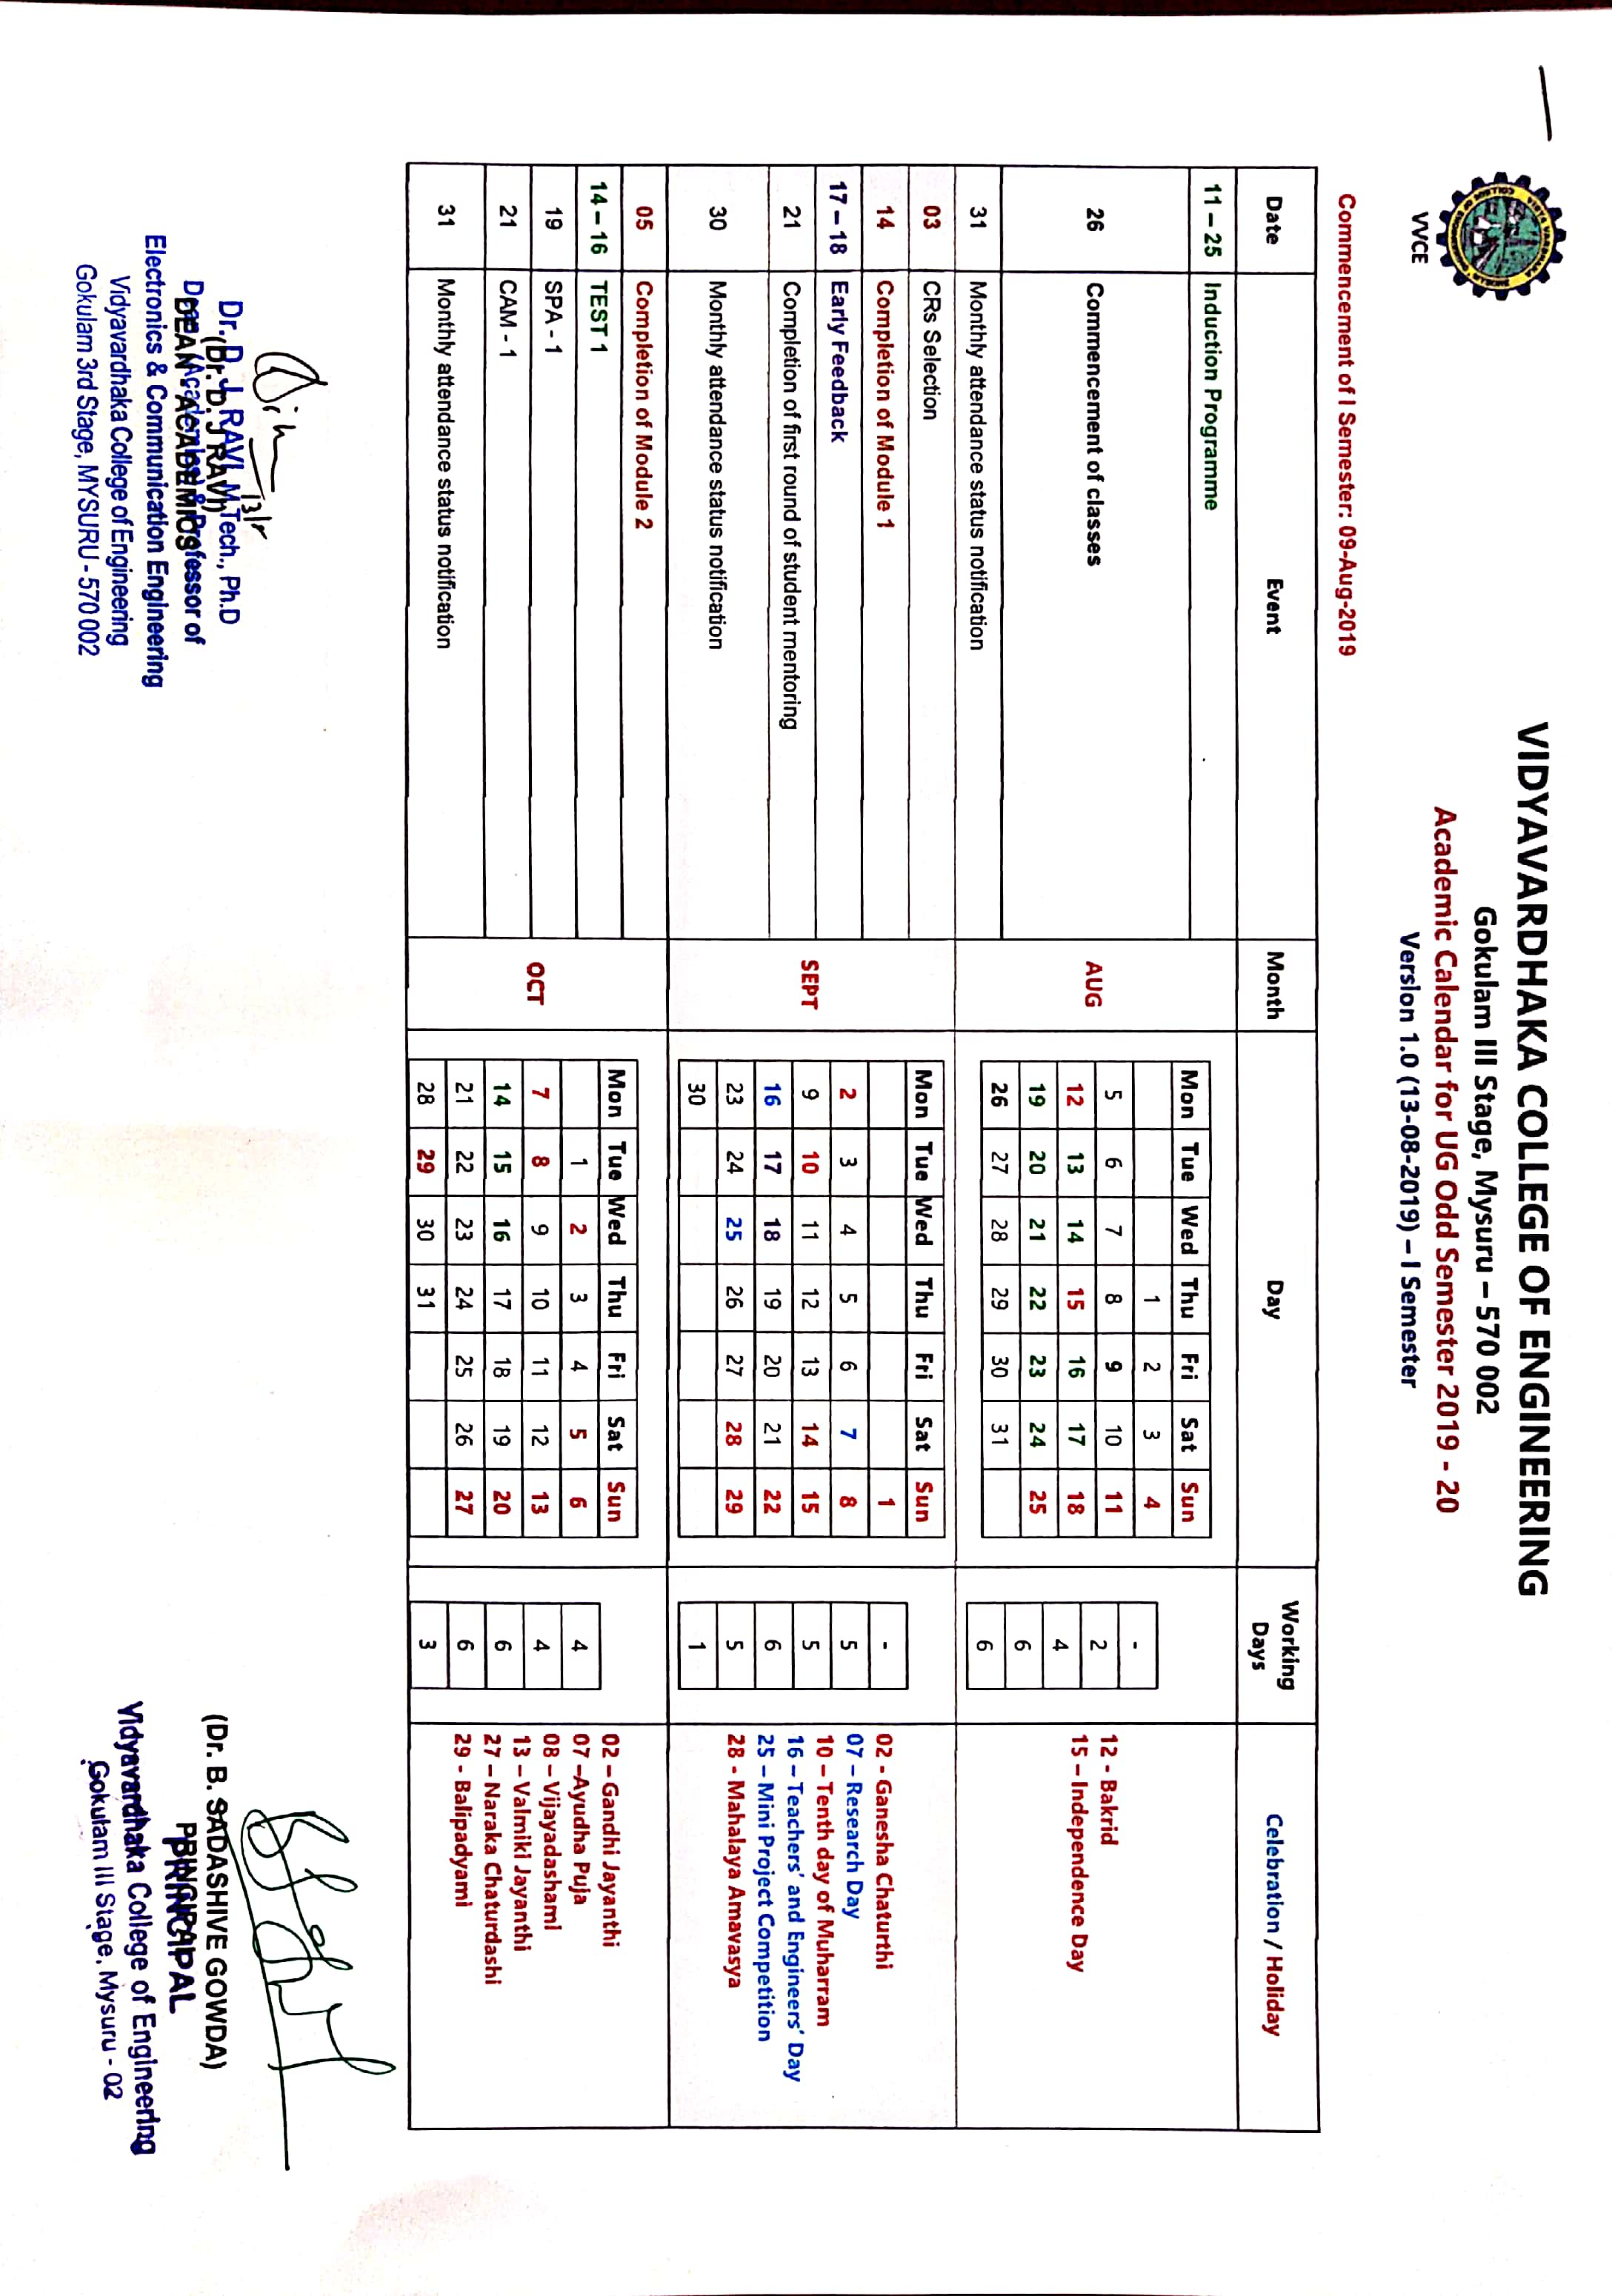
\includegraphics[width=0.20\textwidth]{CoE-1st Sem-Page1.jpg}
	\caption{second figure}
	\label{fig:CoE-1st Sem-Page2}
\end{figure}



\begin{equation}
	a=10
	b=90
\end{equation}



	\[
	a=09+89-67
\]


\begin{equation}
\frac{\sum\frac{a}{\varpi b}}{b-90}
\end{equation}



\subsection{one}
xxxxxxxxxxxxxxxxxxxxxxxxxx kjg  kjhhhhhhhhhhhhhhhhhhhhhhhh jjjjjjjjjjjjjjjjjjjjjjjj jjjjjjjjjjjjjjjjjjjjj
hhhhhhhhhhhhhhhhhhhhhhh hhhhhhhhhhhhhhhh hhhhhhhhhhhhhhhhhhhhhhhhhh hhhhhhhhhhhhhhhhhhhhhhhhhhhhhh




\begin{figure}[h]
	\centering
		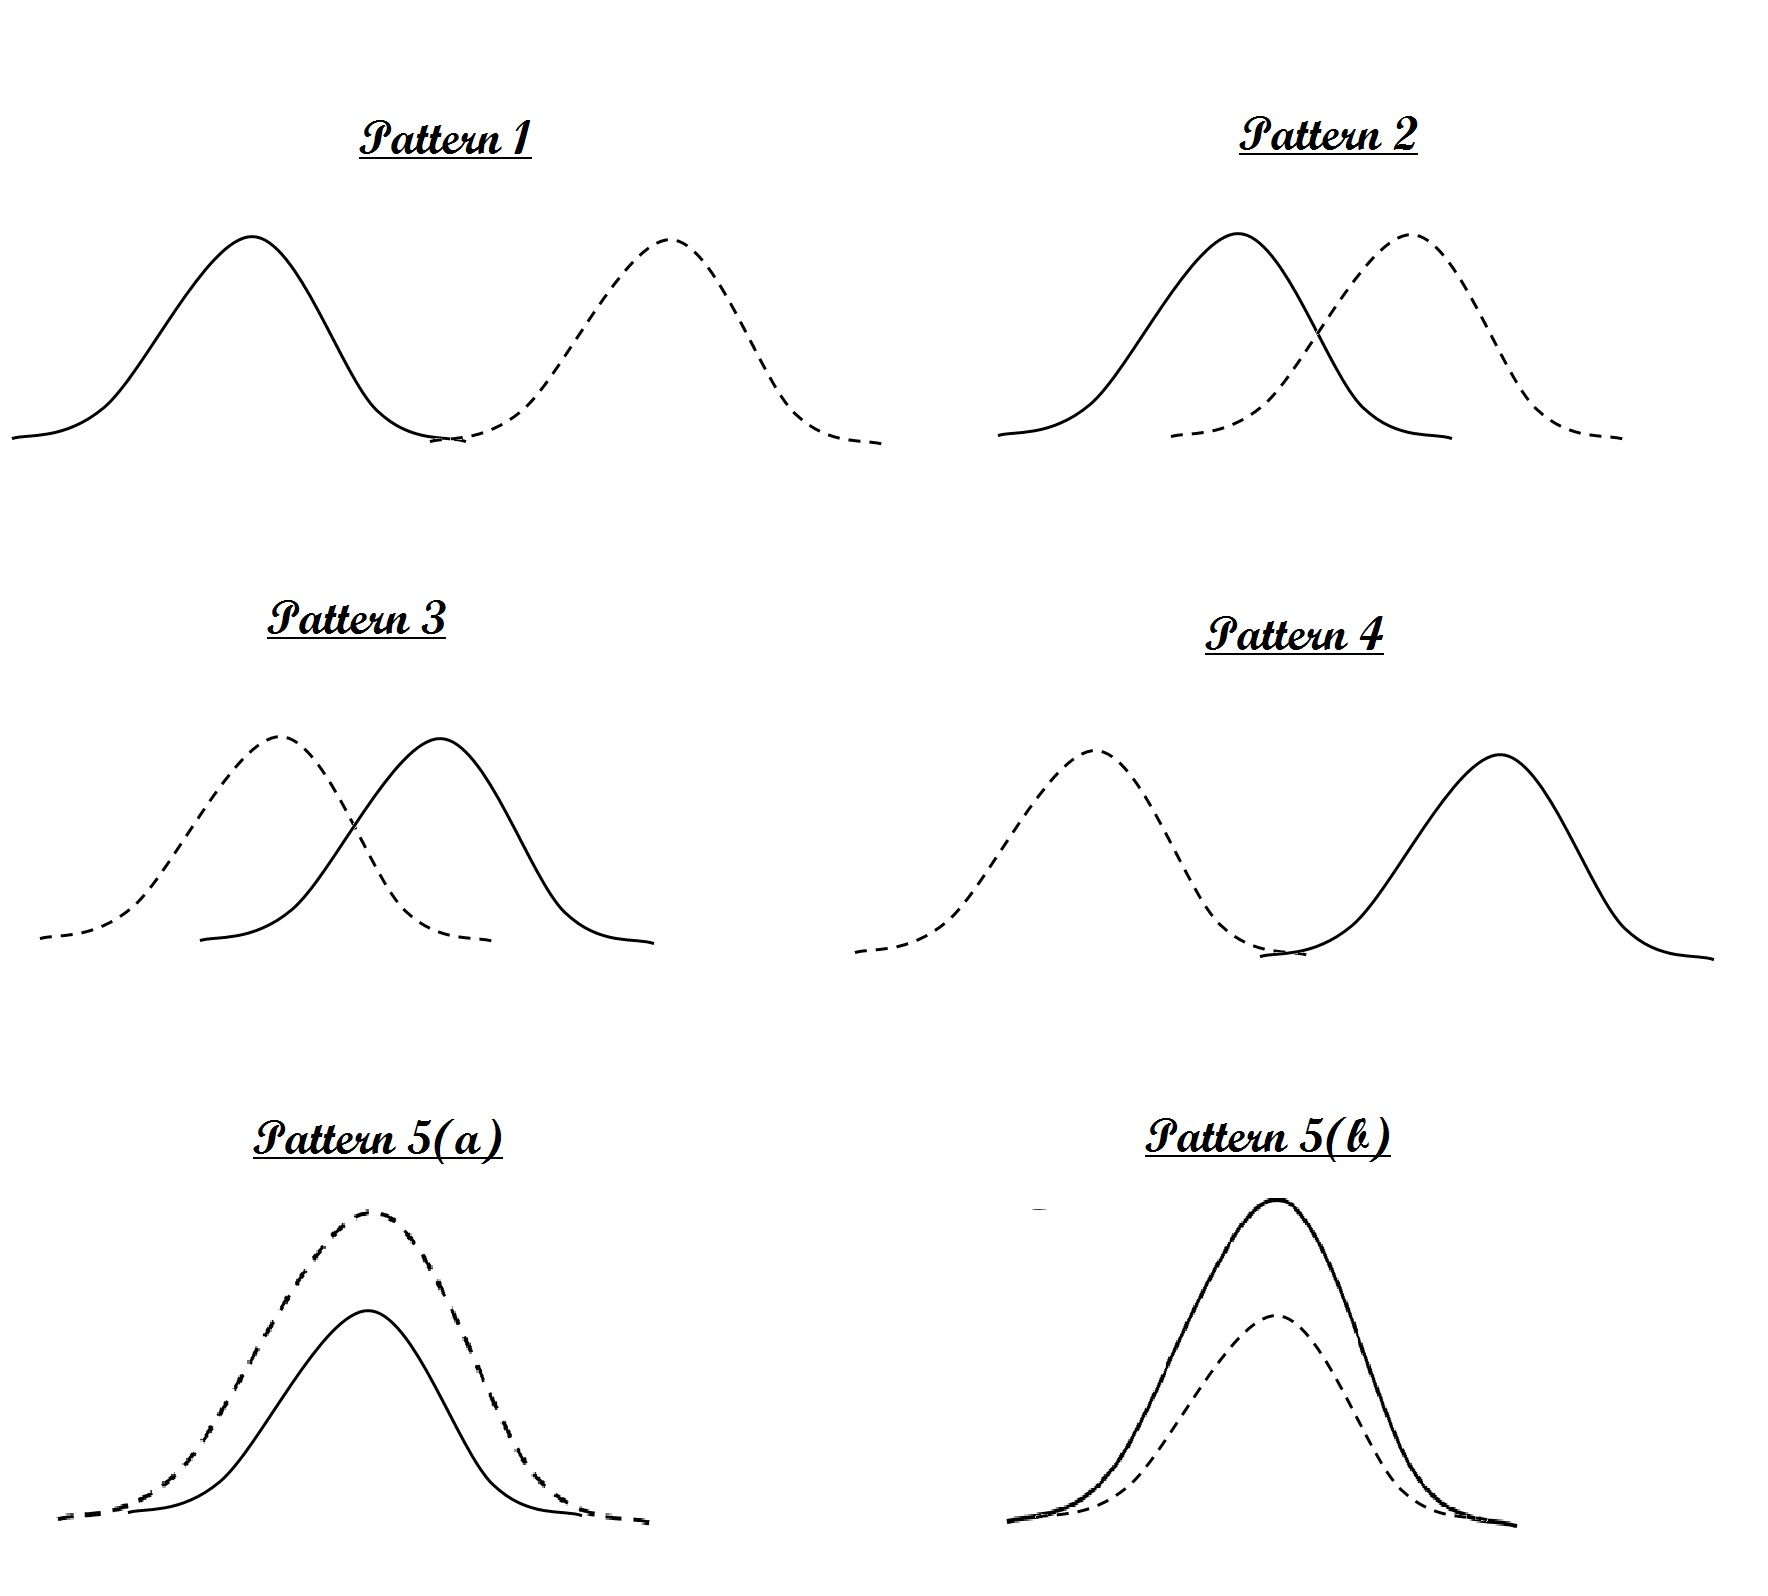
\includegraphics[width=1.0\textwidth]{Normal_Zones.jpg}
	\caption{Possible patterns in “normal- distribution” of medical data samples. Solid line indicates normal (healthy/Non Demented) sample distribution and dotted line indicates abnormal (unhealthy/Demented) sample distribution }
	\label{fNormal_Zones}
\end{figure}






\end{document}




